% header

\documentclass{beamer}
\usepackage[english]{babel}
\usepackage{amsmath,amssymb}
\usepackage[utf8]{inputenc}
\usetheme{Berkeley}

\usepackage{color}
\usepackage{xcolor}
\usepackage{listings}
\usepackage{url}
\usepackage[T1]{fontenc}
\usepackage{xspace}
\usepackage[style=iso]{datetime2}

\usepackage{tikz}
\usetikzlibrary{shapes.callouts,shadows, calc}
\usepackage{listings}


% Solarized colour scheme for listings
%
\definecolor{solarized@base03}{HTML}{002B36}
\definecolor{solarized@base02}{HTML}{073642}
\definecolor{solarized@base01}{HTML}{586e75}
\definecolor{solarized@base00}{HTML}{657b83}
\definecolor{solarized@base0}{HTML}{839496}
\definecolor{solarized@base1}{HTML}{93a1a1}
\definecolor{solarized@base2}{HTML}{EEE8D5}
\definecolor{solarized@base3}{HTML}{FDF6E3}
\definecolor{solarized@yellow}{HTML}{B58900}
\definecolor{solarized@orange}{HTML}{CB4B16}
\definecolor{solarized@red}{HTML}{DC322F}
\definecolor{solarized@magenta}{HTML}{D33682}
\definecolor{solarized@violet}{HTML}{6C71C4}
\definecolor{solarized@blue}{HTML}{268BD2}
\definecolor{solarized@cyan}{HTML}{2AA198}
\definecolor{solarized@green}{HTML}{859900}

% tikz listings support for highlighting - just insert backticks.
\tikzset{note/.style={rectangle callout, rounded corners,fill=gray!20,drop shadow,font=\footnotesize}}    

\newcommand{\tikzmark}[1]{\tikz[overlay,remember picture] \node (#1) {};}    

\newcounter{calloutcounter}
\setcounter{calloutcounter}{1}

\makeatletter
\newenvironment{btHighlight}[1][]
{\begingroup\tikzset{bt@Highlight@par/.style={#1}}\begin{lrbox}{\@tempboxa}}
{\end{lrbox}\bt@HL@box[bt@Highlight@par]{\@tempboxa}\endgroup}

\newcommand\btHL[1][]{%
  \begin{btHighlight}[#1]\bgroup\aftergroup\bt@HL@endenv%
}
\def\bt@HL@endenv{%
  \end{btHighlight}%   
  \egroup
}
\newcommand{\bt@HL@box}[2][]{%
  \tikz[#1]{%
    \pgfpathrectangle{\pgfpoint{0pt}{0pt}}{\pgfpoint{\wd #2}{\ht #2}}%
    \pgfusepath{use as bounding box}%
    \node[anchor=base west,rounded corners, fill=green!30,outer sep=0pt,inner xsep=0.2em, inner ysep=0.1em,  #1](a\thecalloutcounter){\usebox{#2}};
  }%
   %\tikzmark{a\thecalloutcounter} <= can be used, but it leads to a spacing problem
   % the best approach is to name the previous node with (a\thecalloutcounter)
 \stepcounter{calloutcounter}
}
\makeatother


\lstset{
  language=C++,
  basicstyle=\footnotesize\ttfamily,
  rangeprefix=//\ ,
  includerangemarker=false,
}

% Define C++ syntax highlighting colour scheme
\lstdefinelanguage{cpp}{
  language=C++,
  basicstyle=\footnotesize\ttfamily,
  numbers=left,
  numberstyle=\footnotesize,
  tabsize=2,
  breaklines=true,
  escapeinside={@}{@},
  numberstyle=\tiny\color{solarized@base01},
  keywordstyle=\color{solarized@green},
  stringstyle=\color{solarized@cyan}\ttfamily,
  identifierstyle=\color{solarized@blue},
  commentstyle=\color{solarized@base01},
  emphstyle=\color{solarized@red},
  frame=single,
  rulecolor=\color{solarized@base2},
  rulesepcolor=\color{solarized@base2},
  showstringspaces=false,
  moredelim={**[is][\btHL]{`}{`}},
}

\lstdefinelanguage{diff}{
  morecomment=[f][\color{blue}]{@@},           % group identifier
  morecomment=[f][\color{red}]{-},             % deleted lines
  morecomment=[f][\color{green!50!black}]{+},  % added lines
  morecomment=[f][\color{magenta}]{---},       % diff header lines
  morecomment=[f][\color{magenta}]{+++},
}

\lstdefinelanguage{plus}{
  basicstyle=\footnotesize\ttfamily\color{green!50!black},
  emph={see,below,TypeSwitch,unspecified},
  emphstyle=\itshape
}

\lstdefinelanguage{signature}{
  basicstyle=\ttfamily\color{green!50!black},
  emph={see,below,TypeSwitch,unspecified},
  emphstyle=\itshape
}

\newcommand{\desc}[1]{\textit{#1}}
\newcommand{\requires}{\desc{Requires}}
\newcommand{\effects}{\desc{Effects}}
\newcommand{\precondition}{\desc{Precondition}}
\newcommand{\postcondition}{\desc{Postcondition}}
\newcommand{\throws}{\desc{Throws}}
\newcommand{\returns}{\desc{Returns}}
\newcommand{\remarks}{\desc{Remarks}}
\newcommand{\exceptionsafety}{\desc{Exception Safety}}
\newcommand{\fullref}[1]{\ref{#1} \nameref{#1}}

\def\code#1{\texttt{#1}}
\newcommand\mypound{\protect\scalebox{0.8}{\raisebox{0.4ex}{\#}}}
\newcommand{\CC}{C\nolinebreak\hspace{-.05em}\raisebox{0.4ex}{\resizebox{!}{0.6\baselineskip}{\bf++}}}
\newcommand{\cplusplus}{\protect\CC\xspace}
\newcommand{\this}{\code{this}\xspace}
\newcommand{\self}{\code{self}\xspace}
\newcommand{\cvref}{\emph{cv-ref qualifiers}\xspace}
\newcommand{\nl}{\vspace{0.2\baselineskip}}

\title{A Proper Property\\
       \cplusplus Gymnastics with Partially Defined Types}
\author{Gašper Ažman}
\date{November 27, 2017}


\begin{document}

\begin{frame}
  \titlepage
\end{frame}


\section{About: Author}
\begin{frame}
  \frametitle{About Me}
  \begin{itemize}
    \item Gašper Ažman
    \item Started teaching \cplusplus in highschool
    \item Did computer vision research at Berkeley
    \item Helped with Amazon Search Infrastructure at a9.com
    \item Currently at Citadel, building really cool research tools.
    \item A regular at the British Standards Insitute (BSI) Meetings
    \item On the programming committes of CppCon and C$++$Now.
  \end{itemize}
\end{frame}

\section{Disclaimer}

\begin{frame}
\frametitle{Disclaimer}
The opinions in this talk are my own, and do not necessarily reflect the
opinions of Citadel LLC or any of its subsidiaries.\nl

In addition, no Citadel resources were used in the development of this talk.
\end{frame}


\section{Recap}
\begin{frame}[fragile]

\frametitle{So, What is a Property?}
\begin{center}
{\Large A property pretends to be a field.}
\end{center}

Assignment:
\begin{lstlisting}[language=cpp]
airplane.cargo = "hot air";
\end{lstlisting}

Reading:
\begin{lstlisting}[language=cpp]
Payload x = airplane.cargo;
\end{lstlisting}

(Aside: we need a payload, and strings do nicely.)
\begin{lstlisting}[language=cpp]
// books truly are the greatest gift
using Payload = std::string;
using MaybePayload = std::optional<Payload>
\end{lstlisting}

\end{frame}


\begin{frame}[fragile]
\frametitle{Totally.}

\begin{center}
If it quacks like a field, it has to be...
\end{center}

\begin{lstlisting}[language=cpp]
class Airplane {
  MaybePayload cargo;
} airplane;
\end{lstlisting}

\begin{center}
... a field, right?
\end{center}
\end{frame}


\begin{frame}[fragile]
\frametitle{Have you heard of this?}

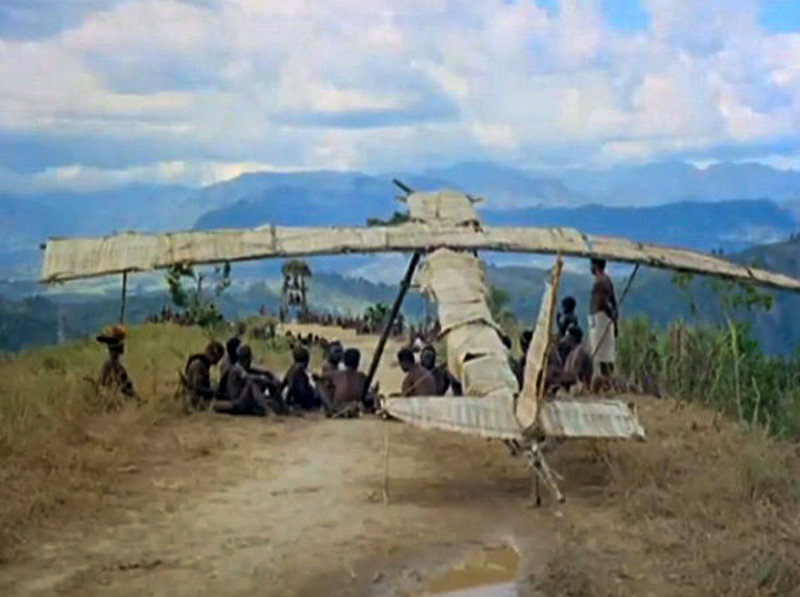
\includegraphics[width=\textwidth]{CargoCultAirplane.jpg}
\end{frame}


\begin{frame}[fragile]
\frametitle{It is only a shell...}

\begin{center}
Instead, it's a pair of a Getter and a Setter on a member.
\end{center}
\begin{lstlisting}[language=cpp]
class Airplane {
  struct Cargo {
    // Setter - assignment from Payload
    void operator=(Payload crate) {
      return {};
    }
    // Getter - implicit conversion to Payload
    operator Payload() const {
      return {};
    }
  };
  Cargo cargo;
} airplane;
\end{lstlisting}
\begin{center}
{\small(We need at least one byte to give \code{cargo} an address)}.
\end{center}
\end{frame}

\section{The Problem}

\begin{frame}[fragile]
  \frametitle{Let's Get More Interesting}
\begin{lstlisting}[language=cpp]
class Airplane {
  MaybePayload `hold`;
public: @\pause@
  struct Cargo {
    MaybePayload operator=(Payload crate) {
      if (!`hold`) {
        @@`hold` = std::move(crate); return {};
      }
      return {std::move(crate)};
    }@\pause@
    operator MaybePayload() {
      return std::exchange(`hold`, {});
    } @\pause@
  } cargo;
} airplane;
\end{lstlisting}
\pause
Pro: this solution is pretty.
\pause

Con: it is not a solution. {\tiny (It does not compile.)}
\end{frame}

\begin{frame}[fragile]
  \frametitle{But... We wants it! We needs it, precious!}

\begin{center}
  {\Huge No.}
  \vspace{.8 in} 

  You're not getting a second breakfast... I mean, a second \this.
\end{center}
\end{frame}


\begin{frame}
  \frametitle{The Problem}

\begin{center}
  {\Huge Get The Host's \this.} \nl

  ... while being reasonably easy to use.
\end{center}
\end{frame}


\section{KISS}

\begin{frame}[fragile]
  \frametitle{Store the \this pointer}
  \begin{lstlisting}[language=cpp]
class Airplane {
  MaybePayload hold;
public:
  struct Cargo {
    MaybePayload operator=(Payload crate) {
      if (!`host`->hold) {
        @@`host`->hold = std::move(crate); return {};
      }
      return {std::move(crate)};
    }
    operator MaybePayload() {
      return std::exchange(`host`->hold, {});
    }
    @@`Airplane* const host`;
  } cargo;
  @@`Airplane() : cargo{this} {}` // every. time.
} airplane;
  \end{lstlisting}
\end{frame}

\begin{frame}[fragile]
  \frametitle{So... How'd we do?}
\begin{center}
{\Huge Poorly.}
\end{center}
\begin{description}
  \item[Needs extra space?] Check.
  \item[Error-prone?] Check.
  \item[No help from C++?] Check.
  \item[Easy?] To understand, yes. To maintain? Good luck.
    (does not pass the WWTDCD\footnote{What Would The Default Constructor Do}
    test)
\end{description}
\end{frame}


\section{Solution Criteria}
\begin{frame}
  \frametitle{Moving the Goalposts Much?}
\begin{center}
{\Huge We need some criteria.}
\end{center}
\end{frame}


\begin{frame}[fragile]
  \frametitle{Criteria}
  \begin{description}
    \item[The First Rule of \cplusplus]\pause
      We only pay for what we use.
    \item[At Most One Macro Per Property]
      The generated code must be contiguous.\pause
    \item[No Pitfalls]
      \begin{itemize}
        \item Easy to read
        \item Easy to write
        \item Easy to modify
      \end{itemize}
  \end{description}
  \begin{center}
    Boils down to \emph{Don't repeat yourself.}\footnote{And we had to repeat
    ourselves with every constructor and assignment operator.}
  \end{center}
\end{frame}


\section{The Idea}

\begin{frame}[fragile]
\frametitle{Member Offsets are Constant}
\begin{center}
  We already have \code{(Cargo*) this}. We can \textbf{compute}
  \code{(Airplane*) this}.
  \includegraphics[width=\textwidth]{offsets.pdf}
\end{center}

\end{frame}


\begin{frame}
  \frametitle{The Anticlimax}
\begin{center}
  I don't think we can get away without macros. \nl \nl \pause

  But, I promise they're not the worst thing about this solution. \nl \nl \pause

  Wait, that's not a good thing. \nl \nl \pause

  ... well, maybe they are.
\end{center}
\end{frame}



\end{document}
